\documentclass[10pt,openright,twoside,french]{book}

\input philippe2013
\input philippe2013_cours
\input philippe2013_sections
\input philippe2013_chapitre

\setcounter{chapter}{6}
\begin{document}

\renewcommand\PartProgramme{Fonctions}
\chapter[Fonctions affines]{Fonctions de référence I\\ Fonctions affines}\label{ch_fonctions_affines}

\section{Variation d'une fonction affine}

\begin{Defi}
    On appelle \iptb{fonction affine}\index{fonction!affine} toute fonction $f$ définie pour tout $x \in \R$ par : \[f(x) = ax + b\] où $a$ et $b$ sont des nombres réels.
\end{Defi}

\begin{Prop}
    Sur un repère orthonormé, la fonction $f \colon x \mapsto ax + b$ est représentée par la droite d'équation $y = ax + b$.
\end{Prop}

\begin{Rmq}[s]
    \begin{itemize}
        \item Si $b = 0$ ($f(x) = ax$), on obtient alors une \iptb{fonction linéaire}\index{fonction!linéaire}. Sa représentation graphique est une droite passant par l'origine. Les fonctions linéaires représentent des situations de proportionnalité.
        \item Si $a = 0$ ($f(x) = b$), on obtient une fonction \iptb{constante} dont la représentation graphique est une droite parallèle à l'axe des abscisses.
    \end{itemize}
\end{Rmq}

\begin{center}
Représentations graphiques :

    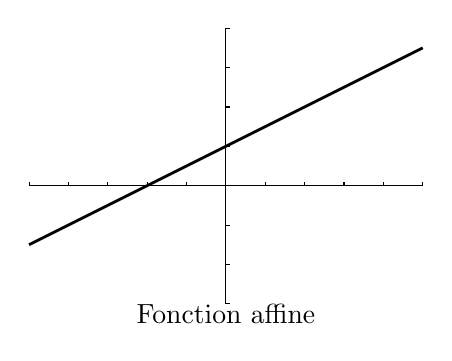
\begin{tikzpicture}[scale=0.5]
        \draw (-5,0) -- (5,0); \foreach \x in {-5,...,5} \draw (\x,0) -- (\x,0.1);
        \draw (0,-3) -- (0,4); \foreach \x in {-3,...,4} \draw (0,\x) -- (0.1,\x);
        \draw[smooth,samples=200,domain=-5:5, line width = 1pt] plot(\x,{0.5*(\x) + 1});
        \draw (0,-3.25) node {Fonction affine};
    \end{tikzpicture}\hfill
    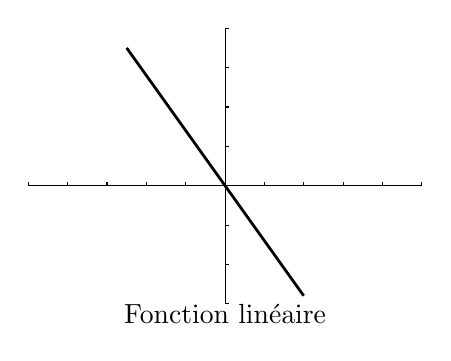
\begin{tikzpicture}[scale=0.5]
        \draw (-5,0) -- (5,0); \foreach \x in {-5,...,5} \draw (\x,0) -- (\x,0.1);
        \draw (0,-3) -- (0,4); \foreach \x in {-3,...,4} \draw (0,\x) -- (0.1,\x);
        \draw[smooth,samples=200,domain=-2.5:2, line width = 1pt] plot(\x,{-1.4*(\x)});
        \draw (0,-3.25) node {Fonction linéaire};
    \end{tikzpicture}\hfill
    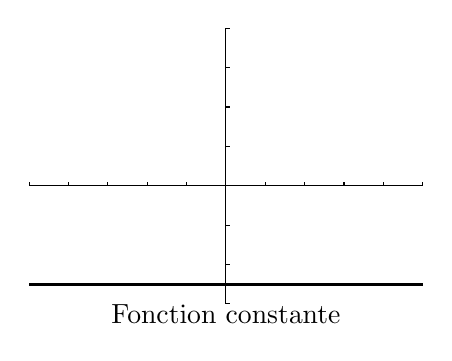
\begin{tikzpicture}[scale=0.5]
        \draw (-5,0) -- (5,0); \foreach \x in {-5,...,5} \draw (\x,0) -- (\x,0.1);
        \draw (0,-3) -- (0,4); \foreach \x in {-3,...,4} \draw (0,\x) -- (0.1,\x);
        \draw[smooth,samples=200,domain=-5:5, line width = 1pt] plot(\x,{-2.5});
        \draw (0,-3.25) node {Fonction constante};
    \end{tikzpicture}
\end{center}

\begin{Exemple}
    Sur un site internet, on peut acheter des blu-ray à \EUR{$15$} l'unité. Les frais de port sont de \EUR{$5$}, quel que soit le nombre de blu-ray acheté.
    \begin{enumerate}
        \item Combien doit-on payer pour $4$ blu-ray achetés ?
        \item Quelle est l'expression de la fonction $P$ donnant le prix total en fonction du nombre $n$ de blu-ray acheté ?
        \item Le prix total est-il proportionnel au nombre de blu-ray acheté ?
        \item La fonction $P$ est-elle une fonction affine ? Pourquoi ?
    \end{enumerate}
\end{Exemple}

On suppose pour la suite $a \neq 0$.

\begin{Thm}
    Soit $f$ la fonction affine définie pour tout $x \in \R$ par $f(x) = ax + b$.
    \begin{itemize}
        \item Si $a > 0$, alors la fonction $f$ est strictement croissante sur $\R$.
        \item Si $a < 0$, alors la fonction $f$ est strictement décroissante sur $\R$.
    \end{itemize}
\end{Thm}\clearpage

\begin{center}
    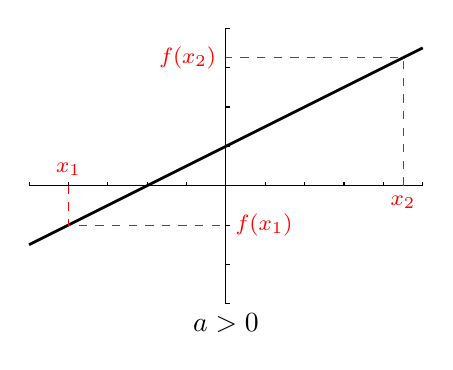
\begin{tikzpicture}[scale=0.5]
        \draw (-5,0) -- (5,0); \foreach \x in {-5,...,5} \draw (\x,0) -- (\x,0.1);
        \draw (0,-3) -- (0,4); \foreach \x in {-3,...,4} \draw (0,\x) -- (0.1,\x);
        \draw[smooth,samples=200,domain=-5:5, line width = 1pt] plot(\x,{0.5*(\x) + 1});
        \draw (0,-3.5) node {$a > 0$};
        \draw[dashed,red] (-4,0) node[above] {\footnotesize $x_1$} -- (-4,-1) -- (0,-1) node[right] {\footnotesize $f(x_1)$};
        \draw[dashed,red] (4.5,0) node[below] {\footnotesize $x_2$} -- (4.5,3.25) -- (0,3.25) node[left] {\footnotesize $f(x_2)$};
    \end{tikzpicture}\hspace{2cm}
    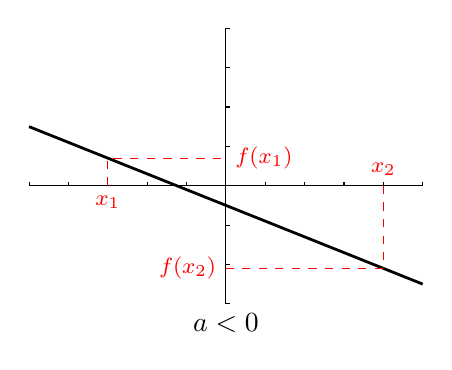
\begin{tikzpicture}[scale=0.5]
        \draw (-5,0) -- (5,0); \foreach \x in {-5,...,5} \draw (\x,0) -- (\x,0.1);
        \draw (0,-3) -- (0,4); \foreach \x in {-3,...,4} \draw (0,\x) -- (0.1,\x);
        \draw[smooth,samples=200,domain=-5:5, line width = 1pt] plot(\x,{-0.4*(\x)-0.5});
        \draw (0,-3.5) node {$a < 0$};
        \draw[dashed,red] (-3,0) node[below] {\footnotesize $x_1$} -- (-3,0.7) -- (0,0.7) node[right] {\footnotesize $f(x_1)$};
        \draw[dashed,red] (4,0) node[above] {\footnotesize $x_2$} -- (4,-2.1) -- (0,-2.1) node[left] {\footnotesize $f(x_2)$};
    \end{tikzpicture}
\end{center}

\begin{Demo}
On considère une fonction affine $f \colon x \mapsto ax + b$ et soient $x_1$ et $x_2$ deux nombres réels.
    \begin{enumerate}
        \item Soit $a > 0$ :
        \[x_1 < x_2 \Rightarrow ax_1 < ax_2 \Rightarrow ax_1 + b < ax_2 + b \Rightarrow f(x_1) < f(x_2).\]
        Ainsi, lorsque $a > 0$, alors $f$ est croissante sur $\R$.
        \item Soit $a < 0$ :
        \[x_1 < x_2 \Rightarrow ax_1 {\color{red}>} ax_2 \Rightarrow ax_1 + b > ax_2 + b \Rightarrow f(x_1) > f(x_2).\]
        Ainsi, lorsque $a < 0$, alors $f$ est décroissante sur $\R$.
    \end{enumerate}
\end{Demo}

\section{Signe d'une fonction affine}

\begin{Thm}
    On rappelle que $a \in \R^*$.\par
    Soit $f$ une fonction affine définie par $f(x) = ax + b$ pour tout $x \in \R$. Alors :
    \[f(x) = 0 \Leftrightarrow x = - \frac b a.\]
    De plus, sur $\intervalleoo{-\infty}{-\frac b a}$, $f$ est de signe constant puis change de signe sur $\intervalleoo{-\frac b a}{+\infty}$.
\end{Thm}

\begin{center}
    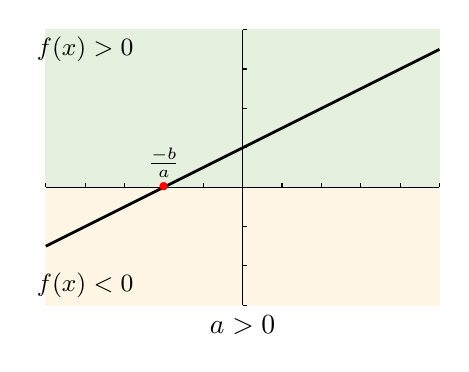
\begin{tikzpicture}[scale=0.5]
        \filldraw[OliveGreen!10] (-5,0) rectangle (5,4);
        \draw (-4,3.5) node {\small $f(x) > 0$};
        \filldraw[Orange!10] (-5,0) rectangle (5,-3);
        \draw (-4,-2.5) node {\small $f(x) < 0$};
        \draw (-5,0) -- (5,0); \foreach \x in {-5,...,5} \draw (\x,0) -- (\x,0.1);
        \draw (0,-3) -- (0,4); \foreach \x in {-3,...,4} \draw (0,\x) -- (0.1,\x);
        \draw[smooth,samples=200,domain=-5:5, line width = 1pt] plot(\x,{0.5*(\x) + 1});
        \draw (0,-3.5) node {$a > 0$};
        \draw (-2,0) node[above] {\footnotesize $\frac{-b}{a}$} node[color=red] {\scriptsize$\bullet$};
    \end{tikzpicture}\hspace{2cm}
    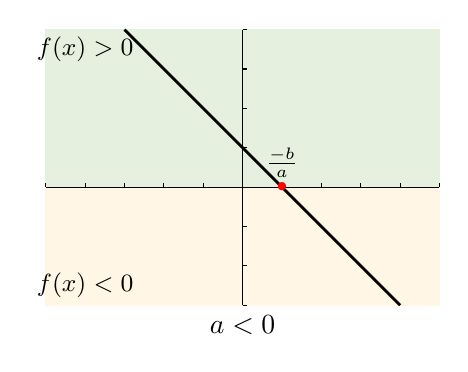
\begin{tikzpicture}[scale=0.5]
        \filldraw[OliveGreen!10] (-5,0) rectangle (5,4);
        \draw (-4,3.5) node {\small $f(x) > 0$};
        \filldraw[Orange!10] (-5,0) rectangle (5,-3);
        \draw (-4,-2.5) node {\small $f(x) < 0$};
        \draw (-5,0) -- (5,0); \foreach \x in {-5,...,5} \draw (\x,0) -- (\x,0.1);
        \draw (0,-3) -- (0,4); \foreach \x in {-3,...,4} \draw (0,\x) -- (0.1,\x);
        \draw[smooth,samples=200,domain=-3:4, line width = 1pt] plot(\x,{-(\x)+1});
        \draw (0,-3.5) node {$a < 0$};
        \draw (1,0) node[above] {\footnotesize $\frac{-b}{a}$} node[color=red] {\scriptsize$\bullet$};
    \end{tikzpicture}
\end{center}

\begin{Demo}
    En effet, $ax + b = 0 \Leftrightarrow ax = -b \Leftrightarrow x = - \frac{b}{a}$.\par
    Le changement de signe est lié au fait que $f$ est soit strictement croissante, soit strictement décroissante.
\end{Demo}

\section{Tableau de variation et tableau de signe}

\begin{center}
\begin{tabular}{c@{\hspace*{0.5cm}}|@{\hspace*{0.5cm}}c}
$f(x) = ax + b$ avec $a > 0$ : & $f(x) = ax + b$ avec $a < 0$ : \\[20pt]
    \begin{tikzpicture}
        \tkzTabInit[nocadre,espcl=2]{$x$/1,Signe de \\ $f$/1.5,Variation de \\ $f$/1.5}{$-\infty$,$-\frac b a$,$+\infty$}
        \tkzTabLine{,-,z,+}
        \tkzTabVar{-/$-\infty$,R,+/$+\infty$}
    \end{tikzpicture}&
    \begin{tikzpicture}
        \tkzTabInit[nocadre,espcl=2]{$x$/1,Signe de \\ $f$/1.5,Variation de \\ $f$/1.5}{$-\infty$,$-\frac b a$,$+\infty$}
        \tkzTabLine{,+,z,-}
        \tkzTabVar{+/$+\infty$,R,-/$-\infty$}
    \end{tikzpicture}
\end{tabular}
\end{center}


\end{document}
